%--------------------------------------------------------------------------
% @file complex_numbers.tex
%
% @date
% @author Martin Noblia
% @email martin.noblia@openmailbox.org
%
% @brief
% Resumen de Numeros complejos
% @detail
%
% Licence:
% This program is free software: you can redistribute it and/or modify
% it under the terms of the GNU General Public License as published by
% the Free Software Foundation, either version 3 of the License, or (at
% your option) any later version.
% 
% This program is distributed in the hope that it will be useful, but
% WITHOUT ANY WARRANTY; without even the implied warranty of
% MERCHANTABILITY or FITNESS FOR A PARTICULAR PURPOSE.  See the GNU
% General Public License for more details.
% 
% You should have received a copy of the GNU General Public License
%
%---------------------------------------------------------------------------
% begin
%-------------------------------------------------------------------------
% Resumen de numeros complejos
%-------------------------------------------------------------------------
\section{Numeros Complejos}
   \subsection{Parte Real e imaginaria}
\begin{defi}
Consideramos a los numeros de la forma: $a+jb$, donde $a$ y $b$ son numeros reales y $j$ es un numero con la propiedad: $j^{2}=-1$. Lo llamaremos numero complejo.
\end{defi}

\begin{ejemplo}
La parte real del numero: $a+jb$, que se anota $Re\{a+jb\}=a$

La parte imaginaria del numero $a+jb$, que se anota $Im\{a+jb\}=b$
\end{ejemplo}
\begin{defi}
   Un numero complejo $z=a+jb$ se puede representar en el plano coordenado mediante el punto $(a, b)$ o mediante una flecha o vector de origen $(0, 0)$ y extremo en $(a, b)$
\end{defi}

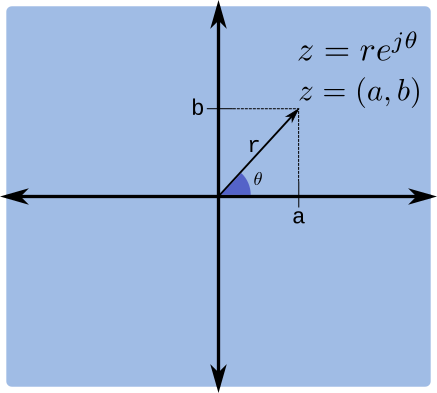
\includegraphics[width=.17\textwidth]{../Algebra/Images/complex_numbers.png}
\subsection{Modulo y argumento de un numero complejo}
\begin{defi}
   El modulo de un numero complejo $z=a+bj$ representa su distancia al origen, y se anota: $|z| = +\sqrt{a^{2}+b^{2}}$
\end{defi}
De lo anterior surge que la distancia entre dos puntos en el plano cartesiano $(a,b)$ y $(c,d)$ se puede calcular: $|(a+bj)-(c+dj)|$
\begin{defi}
   El argumento de un numero complejo $z=a+bj$ es el angulo orientado que forma con el semieje positivo de $x$ y por lo tanto tiene $\infty$ argumentos. Basta elegir uno de ellos que lo llamaremos $\theta$ y todos los demas son : $\theta+2k\pi$ con $k=\pm 1, \pm 2, ...$
\end{defi}
Si $|z|=r$ y $Arg[z]=\theta$ entonces llamaremos al par ordenado $(r, \theta)$ a la representacion del numero complejo $z$ en coordenadas polares. Y como $x=r\cos(\theta)$ e $y=r\sin(\theta)$ se conoce como la representacion trigonometrica $z=r(\cos(\theta)+ j\sin(\theta))$.

\begin{defi}{Potencias:}
   Dado un numero complejo $z=r(\cos(\theta)+j\sin(\theta))$ sus potencias son:
   \begin{equation}
      z^{n} = r^{n}(\cos(n\theta)+j\sin(n\theta))
   \end{equation}
\end{defi}


La representacion trigonometrica nos ayuda a entender el producto y el cociente de los numeros complejos.
\begin{align}
   z_{1}z_{2} &= r_{1}(\cos(\theta_{1})+j\sin(\theta_1))r_{2}(\cos(\theta_{2})+j\sin(\theta_{2}))\\
   z_{1}z_{2} &= r_{1}r_{2}[(\cos(\theta_1)\cos(\theta_2)-\sin(\theta_1)\sin(\theta_2))+j(\cos(\theta_1)\sin(\theta_2)+\cos(\theta_2)\sin(\theta_1))]\\
   z_{1}z_{2} &= r_{1}r_{2}[\cos(\theta_1 + \theta_2)+j(\sin(\theta_1 + \theta_2))]
\end{align}

\begin{defi}
   El modulo del producto es el producto de los modulos: $|z_1 z_2|=|z_1||z_2|$
\end{defi}

\begin{defi}
   Un argumento (ya que hay $\infty$) del producto es la suma de los argumentos: $Arg(z_1 z_2)=Arg(z_1)+Arg(z_2)$
\end{defi}

\begin{defi}{Raices n-esimas de la unidad:}
   En general se tienen $n$ raices n-esimas de la unidad, ya que $z^{n} = r^{n}(\cos(n\theta)+j\sin(n\theta))=1$ entonces $r=1$ y $n\theta=2k\pi$
   Tomando sucesivamente $n=0,1,2,3,...,n-1$ encontramos las $n$ raices $\cos(\frac{2k}{n}\pi)+j\sin(\frac{2k}{n}\pi)$ que son potencias sucesivas de:
   $\omega = \cos(\frac{2}{n}\pi)+j\sin(\frac{2}{n}\pi)$. Se disponen como vertices de un poligono regular de $n$ lados inscriptos dentro de la circunferencia unidad
\end{defi}

\begin{defi}{Raices de un numero:}
   Sea $\omega=r(\cos(\theta)+j\sin(\theta))$ si $z=s(\cos(\theta)+j\sin(\theta))$ es una raiz n-esima de $\omega$ tenemos:
   $z^{n}=s^{n}(\cos(n\phi)+j\sin(n\phi))=r(\cos(\theta)+j\sin(\theta))$. De donde se obtiene que $s^{n}=r$ entonces $s=r^{1/n}>0$ y 
   $n\phi=\theta + 2k\pi$ con $k$ entero.
   
   Luego: $\phi=\frac{\theta}{n}+\frac{2k\pi}{n}$ con $k=0,\pm 1,\pm 2,\pm 3...,\pm (n-1)$. para $k=0,1,2,3,...,n-1$ obtenemos $n$ raices distintas:

   \begin{equation}
      z_{k}=r^{1/n}(\cos(\frac{\theta + 2k\pi}{n})+j\sin(\frac{\theta + 2k\pi}{n}))
   \end{equation}
\end{defi}

%---------------------------------------------------------------------------
% end
%---------------------------------------------------------------------------
